 % Describes how we find the peaks/clusters in the data (Maarten de Waard will
 % fill this in)
 This section will discuss how we find clusters in sessions. A cluster is a 
part of a sessions in which the bird shows one type of behavior. Once we have
clusters we can annotate quickly and learn per cluster.

We approached this problem in two different manners. First we simply looked at
change in the acceleration. We spent a lot of time tweaking and optimizing the parameters
to find better clusters but in the end we had to conclude that this would never work. 
The second
approach has it's origins in `computer vision' % Is dit waar!?
and works with histograms to 
match standard behaviour to parts of sessions.

\subsection{The First Approach: Finding Peaks in Acceleration}
 Probably the most important of the GPS data we get from \bits are the X and Y
 position and speed of the bird. There are two speed entries in the database we
 use. The first we use is `instantaneous speed'.    
This the speed the bird has on the time of
 connecting to the GPS, calculated from two subsequent measurements. The second
we use is 
 `trajectory speed'. This is speed calculated from two GPS locations. 
We decided to use the latter because it has a smaller error rate. 
 Our assumption was that we could cluster the data well 
 enough by only looking at speed differences. Figure \ref{fig:speed} shows
 why.
 % TODO: Dit figuurtje maken. Ik kom er namelijk net achter dat de derivative
 % misschien niet exact doet wat we willen, omdat het speed1 en speed2 apart van
 % elkaar gebruikt. Een goeie hiervoor is device_535, sessie_000.

\begin{figure}
  \centering
  \subfloat[Speed of the bird.]{\label{fig:speed1}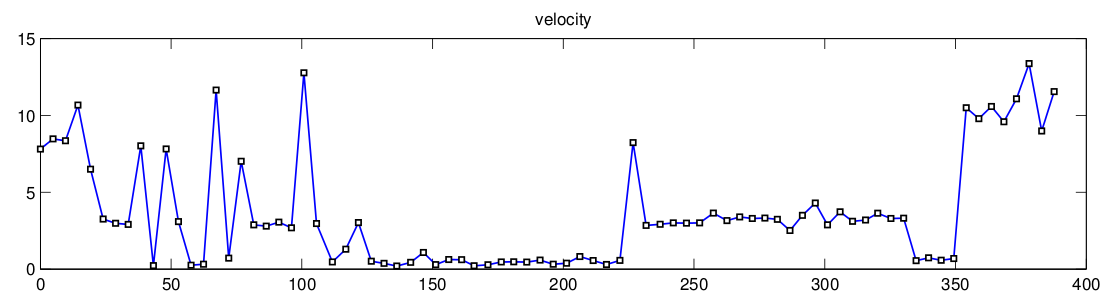
\includegraphics[width=0.8\textwidth]{speed1.png}} \\
  \subfloat[Difference in speed.]{\label{fig:speed2}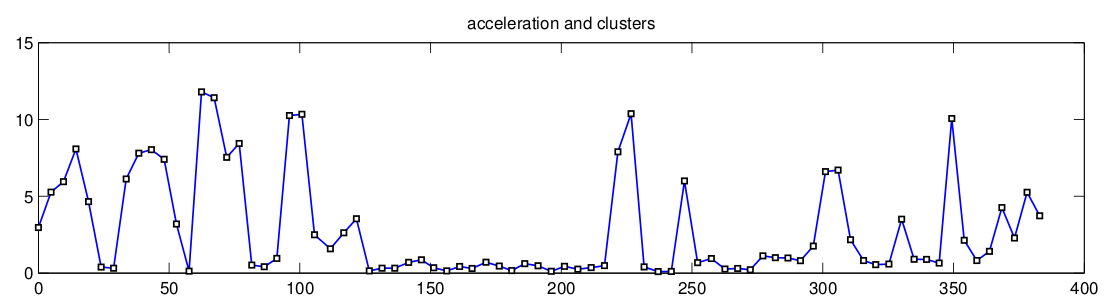
\includegraphics[width=0.8\textwidth]{speed2}} \\
  \caption{The difference is absolute because this makes finding peaks easier. The difference is sometimes a bit higher while the speed does not seem to differ at all. This means the bird changed directions.}
  \label{fig:speed}
\end{figure}

%\begin{figure}
%\centering
%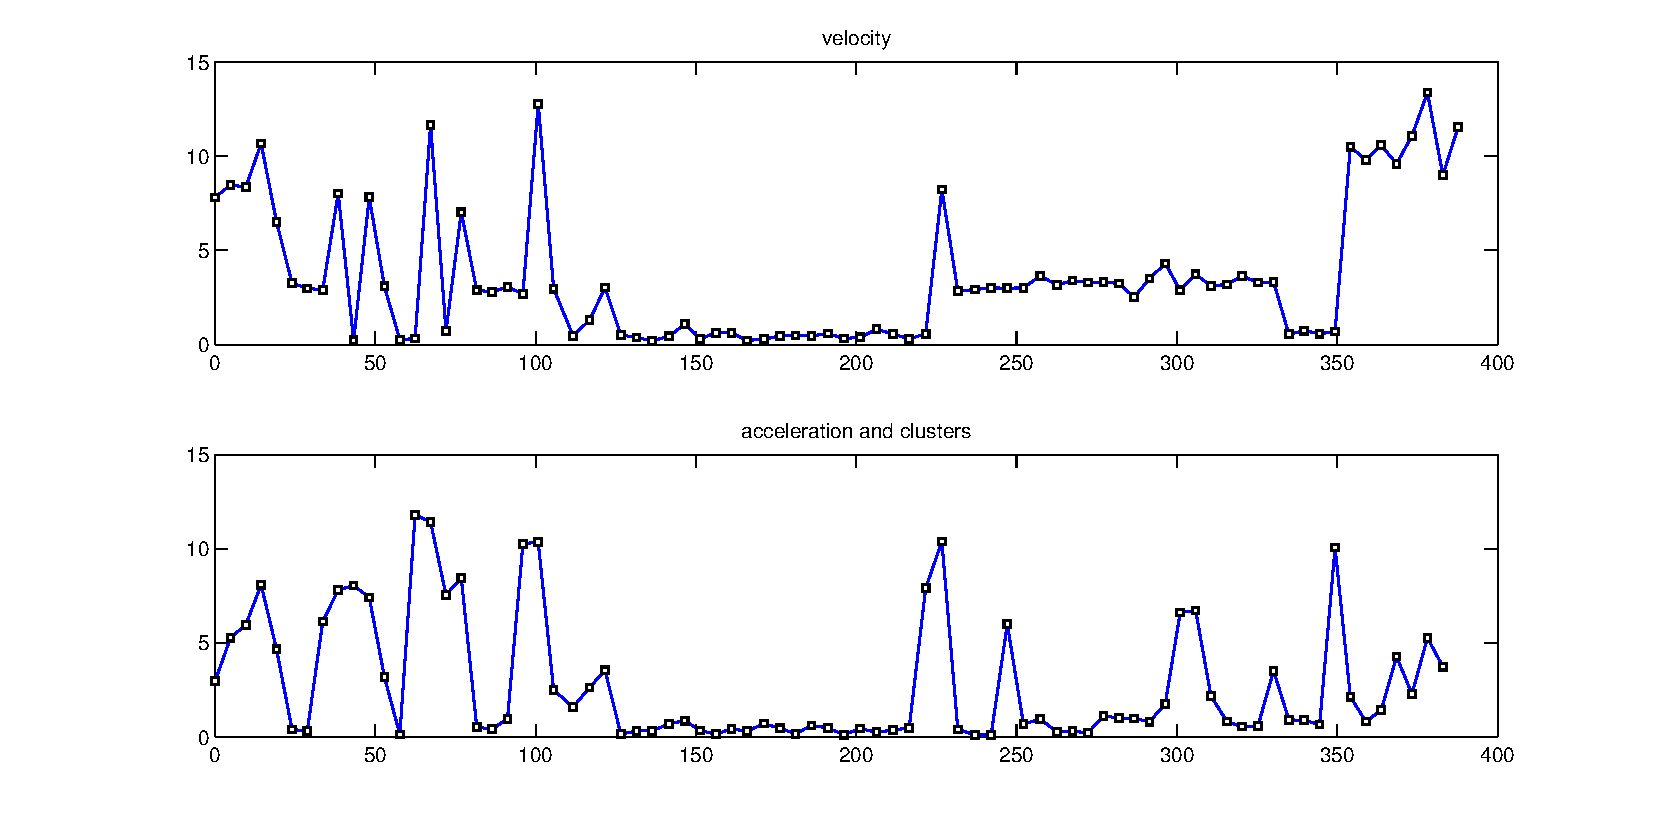
\includegraphics[width=.8\textwidth]{speed.pdf}
%\caption{The speed of the bird (above) and the difference in speed (under). As
%you can see, the difference is absolute (because this makes finding peaks
%easier). The difference is some times a bit higher, while the speed does not
%seem to differ at all. This means the bird changed his direction.}
%\label{fig:speed}
%\end{figure}

As can be seen, the speed-difference is low on points where the bird is assumed
to be flying or sitting on the water. In other points the speed differs a lot.
On these places we can assume that the bird is foraging.


\subsubsection{Finding the Peaks}
 Clustering, in our case, starts with finding peaks in these speed differences.
 The peaks indicate a change in the bird's behavior, or indicate that the bird
 is foraging. Finding these peaks is done in two steps:

 \begin{itemize}
    \item Check where the value of the speed difference is bigger than a certain
    threshold.
    \item Loop through these differences and place a marker before the threshold
    is crossed upwards, or after it has been crossed downwards. 
 \end{itemize}
 
 This creates a representation of a peak by marking its left and right side.
 This has the advantage that we do not get these speed differences in our
 clusters as they would add noise to the learning data.

 \subsubsection{Grouping the Peaks}
 For grouping peaks, we created another algorithm. This algorithm looks at three
 characteristics.  
 \begin{itemize}
 \item The time elapsed between two peaks
 \item The difference between the current time elapsed between peaks, and the
 current cluster's average
 \item The difference between the time elapsed between the first peak of the
 cluster, and the average of the rest of the cluster.
 \end{itemize}
 This way we can find the `chaos clusters', because the time between the peaks
 in these clusters is always between a certain threshold (currently set on
 \timeThreshold seconds). 
 When a peak is too far from the  current average, this almost always indicates
 a change in behavior, so a new cluster should be started.this is done by the
 second and third characteristic specified above.

It turned out however the data is too chaotic too group well in every situation. 
Also the difference between high and low resolution turned out to be troublesome. It
could not be done. We abandoned this train of thought and picked a more sophisticated 
method.


%%%%%%%%%%%%%%%%%%%%%%%%%%%%%%%%%%%%%%%%%%%%%%%%%%%%%%%%%%%%%%%%%%%%%%%%%%%%%%%%%%%
%%%%%%%%%%% AWESOME HISTOGRAM SUBSECTION BEGINT HIER
%%%%%%%%%%%%%%%%%%%%%%%%%%%%%%%%%%%%%%%%%%%%%%%%%%%%%%%%%%%%%%%%%%%%%%%%%%%%%%%%%%%


\subsection{The Second Approach: The Use of Histograms}
\begin{figure}
  \centering
  \subfloat[Model for floating.]{\label{fig:clusteringRaw}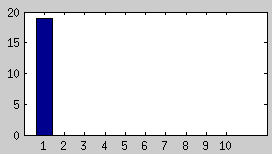
\includegraphics[width=0.3\textwidth,height=1in]{bar1speed}} 
  \subfloat[Model for flying.]{\label{fig:clusteringInterpolated}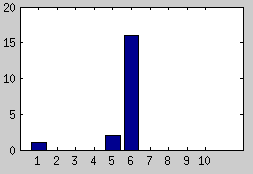
\includegraphics[width=0.3\textwidth,height=1in]{bar2speed}} 
  \subfloat[Model for hunting.]{\label{fig:clusteringHists}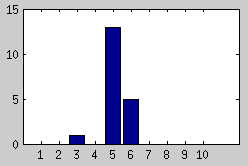
\includegraphics[width=0.3\textwidth,height=1in]{bar3speed}}
  \caption{Histograms that count the speed for the models of the three
  behaviors, using the following bins: [0, 1, 2, 4, 5, 10, 20, 40, 60, 120]}
  \label{fig:modelHistogramsSpeed}
\end{figure}
\begin{figure}
  \centering
  \subfloat[Model for
  flying.]{\label{fig:clusteringRaw}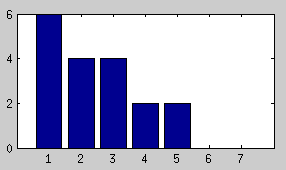
\includegraphics[width=0.3\textwidth,height=1in]{bar2angle}} 
  \subfloat[Model for hunting.]{\label{fig:clusteringInterpolated}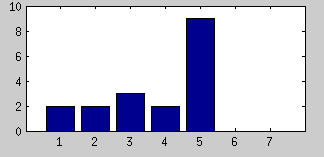
\includegraphics[width=0.3\textwidth, height=1in]{bar3angle}} 
  \caption{Histograms that count the angle for the models of flying and hunting,
  using the following bins: [0, 5, 10, 30, 60, 180, 360]. There is no model for
  floating, because  the direction of floating could not be measured properly
  using instantaneous speed.}
  \label{fig:modelHistogramsAngle}
\end{figure}
This different version works on another basis: We create two histograms. One
contains the trajectory speeds of the bird and the other contains the
difference in the angle of the instantaneous speeds. This means that we count
how many times the speed or angle is between certain values, and represent that
in an array with these counts. For further illustration see figure
\ref{fig:modelHistogramsSpeed} and \ref{fig:modelHistogramsAngle}.


We take an example of each kind of behavior (floating, flying and foraging).
This example can be compared with a bit of the data we are
clustering. For this we loop over the session data, each time selecting
\windowSize.

This method consists of five steps:
\begin{itemize}
    \item Interpolating the values
    \item Creating the histograms
    \item Comparing the histograms
    \item Smoothing the histogram values
    \item Finding the clusters
\end{itemize}

Using these steps, the program can loop over the session data, using a certain time
window. Histograms made from the time window can then be compared to the
histograms of the examples (which equally sized) and a
percentage of how different they are can be calculated. The session can now be clustered by
adding cluster beginnings and endings where the values of the histogram
differences (so the values in figure \ref{fig:clusteringHists}) cross each
other. The histogram that has the highest values, is also put in our feature
vector for learning purposes.

\begin{figure}
  \centering
  \subfloat[Raw data of a session.]{\label{fig:clusteringRaw}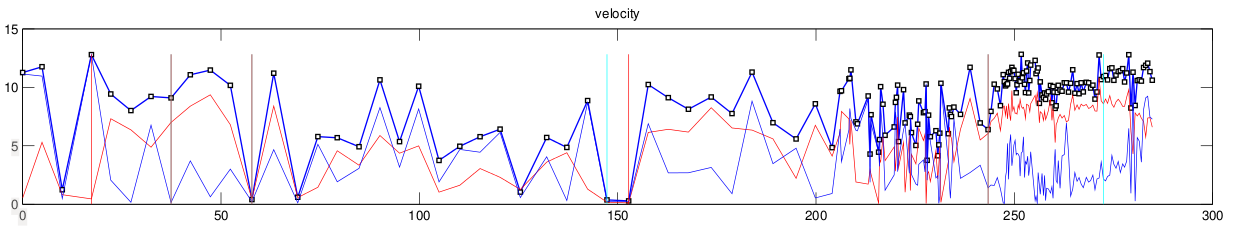
\includegraphics[width=0.8\textwidth]{clustersHists1}} \\
  \subfloat[Interpolated data of a session.]{\label{fig:clusteringInterpolated}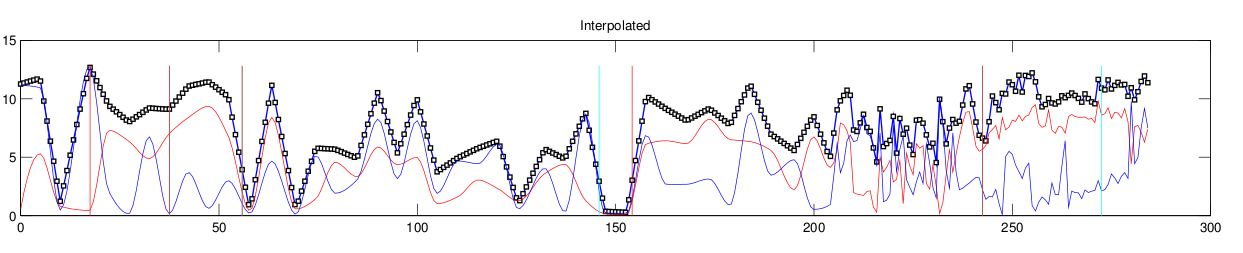
\includegraphics[width=0.8\textwidth]{clustersHists2}} \\
  \subfloat[Similarity of the flight to behavior percentages. Red indicates floating, green flying and blue hunting.]{\label{fig:clusteringHists}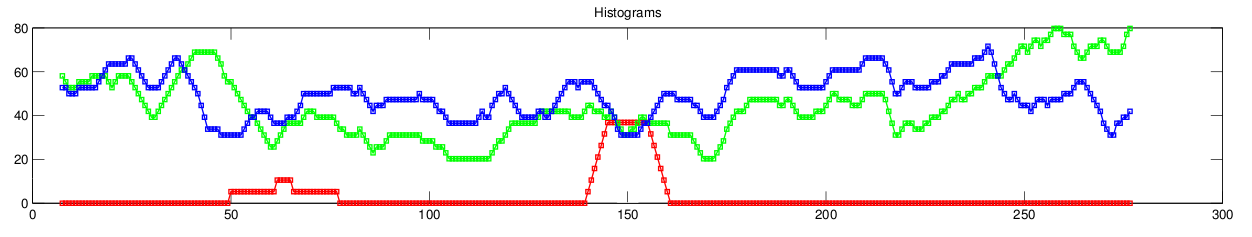
\includegraphics[width=0.8\textwidth]{clustersHists3}}
  \caption{Different plots of the clustering process. Red vertical bars indicate
  beginnings of clusters. Cyan vertical bars indicate ends of clusters.}
  \label{fig:clustering}
\end{figure}

\subsubsection{Interpolating the Values}
The data consists of sessions with different resolutions. Even during the
session, the resolution can differ. This
would mean that when we are looking at high resolution data, and we compare it
with a low resolution example, calculating an accurate difference value between
two histograms would get very difficult. Therefore
we need to have exactly as many data points in the example, as in the current 
histogram. 

This is easily achieved by interpolating the data. Since \matlab has integrated
interpolation functions, we have chosen to interpolate with `Piecewise Cubic
Hermite Interpolating Polynomial (PCHIP)', which is a bit more computationally
expensive than linear interpolation, but returns a smoother curve. 

\subsubsection{Creating the Histograms}
%How we cretae heistrioangsams:
In \matlab, creating histograms is not a problem. The function \texttt{histc} is
used, and returns a division of the data, over the specified bins. A histogram
in \matlab is formatted like a 1 by N matrix. These
histograms can be compared as described in the next part.

\subsubsection{Comparing the Histograms}
Equation \ref{eq:diff} compares two algorithms, and returns a value closer to
zero when the histograms are the same, going up when they differ more.
\begin{equation}
\label{eq:diff}
Diff = \sum ( \left| exampleHistogram - currentHistogram \right| ) \vspace{10pt}
\end{equation}
 
Because the maximum value of $Diff$ depends on the time window, the program converts
it to percentages. That is done with equation \ref{eq:perc}, where the sum of a
histogram is the same as the number of entries it has.

\begin{equation}
\label{eq:perc}
percentage = 100 - \frac{Diff}{2 \sum Histogram} \times 100
\end{equation}

Now we have a percentage for each point, of how much it resembles each behavior.
A plot of this percentage is shown in figure
\ref{fig:clusteringHists}.
This can be used to find clusters, because each time this differs, a new
cluster can be assumed to be starting.

\subsubsection{Smoothing the Histogram Values}
After the previous step, the data sometimes has only one or two points above the
others, during a cluster. This could be due to a gps error or a sudden movement
of the bird. We do not want to see this as a new cluster, so the data should be
smoothed.

This is done in a simple and elegant way. A window of (in our case) 7 points is
moved over the data. The mode of these points should be the value of the middle
of the seven. This way, if less than four of the points have another value than
their surroundings, there are too little points to create a new cluster, and the
difference was probably noise. 

\subsubsection{Finding the Clusters}
In this smoothed data, the clusters can easily be found. The program saves the
timestamp of each time the histogram values differ, this way returning a matrix
with two columns: Begin time, and end time. 

The clusters shorter than 15 minutes, are deleted. Allthough
this has as a result that we do not use all the data for learning, this does
select the best usable data, and uses that. the clusters of approximately 5 to
15 minutes would be worthless learning data, because they are too short to
depict actual behavior.
